\chapter{Incoherent Scatter Radar Signal Model \& Processing}
\label{chapter:isrproc}
\thispagestyle{myheadings}

% set this to the location of the figures for this chapter. it may
% also want to be ../Figures/2_Body/ or something. make sure that
% it has a trailing directory separator (i.e., '/')!
\graphicspath{{2_ISRProc/Figures/}}

%%%%%%%%%%%%%% Intro %%%%%%%%%%%%%%%%%%%%%%%%%%%%%%%%%%%%%

This chapter will give the background on the signal model and processing aspects of ISR. The first section will explore the physical  underpinning of the incoherent scatter signal from the ionosphere. The second section will detail the basics of radar processing and how the different types of measurements are made. In the final section of this chapter the specific processing that takes place in an ISR will be detailed.

\section{Incoherent Scatter}
\label{sec:incohscat}
When electrons are freed from their bonds as in a plasma they can oscillate in a manner modeled as a dipole antenna. If an electromagnetic wave, such as one from a radar pulse, impinges on these electrons they will accelerate and re-radiate a wave. This scattering process is known as Thomson scatter \cite{Hutchinson_2002}. This radiation, when taken as a collection of scatterers from a large set of electrons, varies in time $t$, with fluctuations in electron density $n_e(\mathbf{k},t)$, where $\mathbf{k}$ is the Bragg vector \cite{kudeki:milla:1}. In the far-field condition the Bragg vector is defined as
\begin{equation}
\label{eqn:bragg}
\mathbf{k}=\mathbf{k}_s-\mathbf{k}_i,
\end{equation}
where $\mathbf{k}_s$ and $\mathbf{k}_i$ are the wavenumbers for scattered and incident waves respectively \cite{sheffield2010}. The Bragg vector is the frequency parameter in $n_e(\mathbf{k},t)$, where the spatial Fourier transform $n_e(\mathbf{r},t)$ has position vector $\mathbf{r}$. As these charges move the scattered waves are given a Doppler shift based off of their velocity, $\mathbf{v}$ along the Bragg vector. This Doppler shift in frequency can be represented as
\begin{equation}
\label{eqn:dop1}
\omega=\mathbf{k} \cdot \mathbf{v},
\end{equation}
where $\omega$ is the frequency shift from the velocity along the Bragg vector \cite{sheffield2010}. $n_e(\mathbf{k}, \omega)$ can be thought of as both the Fourier Transform along time of $n_e(\mathbf{k},t)$ and the collective Doppler spectrum from the density at a specific Bragg vector $\mathbf{k}$.

These fluctuations are driven by the random thermal motions of the electrons and the collective radiation they create is known as incoherent scatter \cite{kudeki:milla:1}. Another term for this is \textit{non-collective} scattering with relation,
\begin{equation}
\label{eqn:incohorig}
k*\lambda_{e} << 1,
\end{equation}
where $\lambda_{e}$ is the electron Debye length, and $k=|\mathbf{k}|$. This will cause the spectrum to show the collective effects of the velocity distribution of the particles \cite{sheffield2010}.
Although the scattering is driven through a random process it reveals several pieces of information about a plasma, especially in the ionosphere. Due to the electrical interaction between the ions and electrons a correlation structure develops, creating a shaped Doppler spectrum that a radar can detect. This Doppler spectrum is a power spectral density estimate of the electron density fluctuations across time $t$ and $\langle \left|n_e(\mathbf{k},\omega)\right|^2\rangle$.

There have been a number of derivations of this process since the development of ISR \cite{dougherty:farley1960,farleydougherty:ISR2,doughteryfarley:ISR3,hagfors1961}. This thesis uses the formulation from~\cite{kudeki:milla:1,kudeki:milla:2,Kudeki:2006kx}
\begin{equation}
\label{eq:mainspeceq:body}
\langle \left|n_e(\mathbf{k},\omega)\right|^2\rangle = \frac{|j\omega\epsilon_0 + \sigma_i|^2 \langle |n_{te}(\mathbf{k},\omega)|^2\rangle}{|j\omega\epsilon_0 +\sigma_e+\sigma_i|^2} + \frac{| \sigma_e|^2 \langle |n_{ti}(\mathbf{k},\omega)|^2\rangle}{|j\omega\epsilon_0 +\sigma_e+\sigma_i|^2}.
\end{equation}
The full derivation of~\eqref{eq:mainspeceq:body} is given in Appendix~\ref{appendix1}.
An example of this spectrum, with a $|\mathbf{k}|=18.5$ rad/m and using parameters representative of the F-region ionosphere, is shown in Figure \ref{fig:ispecch2}. 
% make ISR spectra
\begin{figure}[!t]
\centering
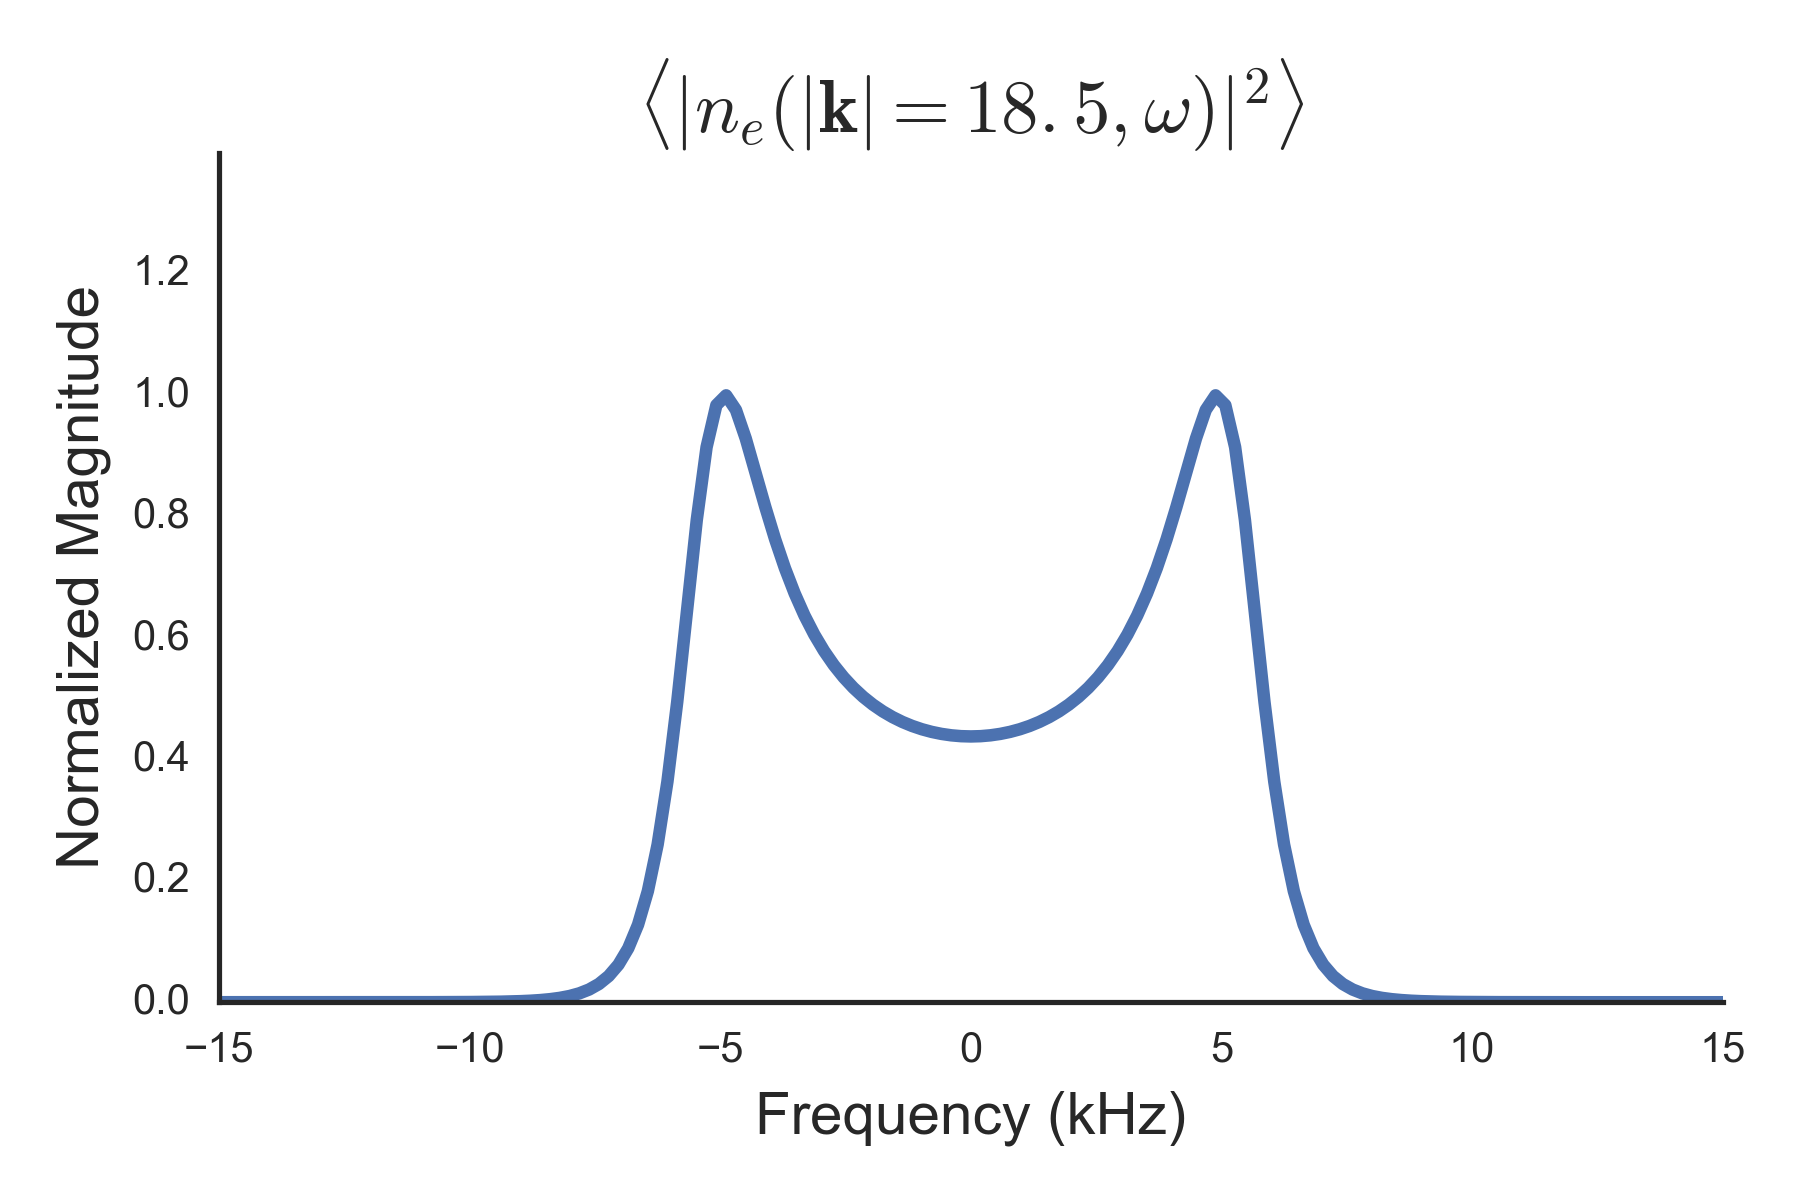
\includegraphics[width=4in]{Specion}
\caption{IS spectrum ion line with all O$^+$ ions, $N_e = 10^{11}$, $T_e=2500 ^\circ$ K and $T_i=1000 ^\circ$ K. }
\label{fig:ispecch2}
\end{figure}
The IS spectrum has a number of different sections separated in frequency.
This thesis focuses on the ``ion line'' shown in Figure~\ref{fig:ispecch2}. This naming is due to the IS spectrum revealing a damped version of ion acoustic waves
\begin{equation} 
\label{eqn:ial}
\omega=k_0\sqrt{\frac{K_b(T_e+3T_i)}{m_i}}
\end{equation}
where $k_0$ is the wavenumber, $\omega$ is the radian frequency of the wave, $K_b$ is Boltzman's constant, $m_i$ is the mass of the ion species and $T_e$ and $T_i$ are the temperatures of the electron and ions \cite{chen1984introduction}. 
The ion acoustic mode returns the most power and can give information on both electron and ions, so it is commonly used in ISR analysis.

As its name implies, IS is inherently stochastic in nature. To measure this spectrum with usable error margins a number of samples of this process must be averaged together \cite{Diaz:2008co}. Common ISR analysis practice refers to samples of this random process as "pulses" to distinguish this from samples in signal processing applications \cite{dtsp:openhiem}. A demonstration of the convergence of a measurement going to the spectrum, using a periodogram estimator \cite{kay1988modern}, is depicted in Figure \ref{fig:ispecch2ave}.
\begin{figure}[!t]
\centering
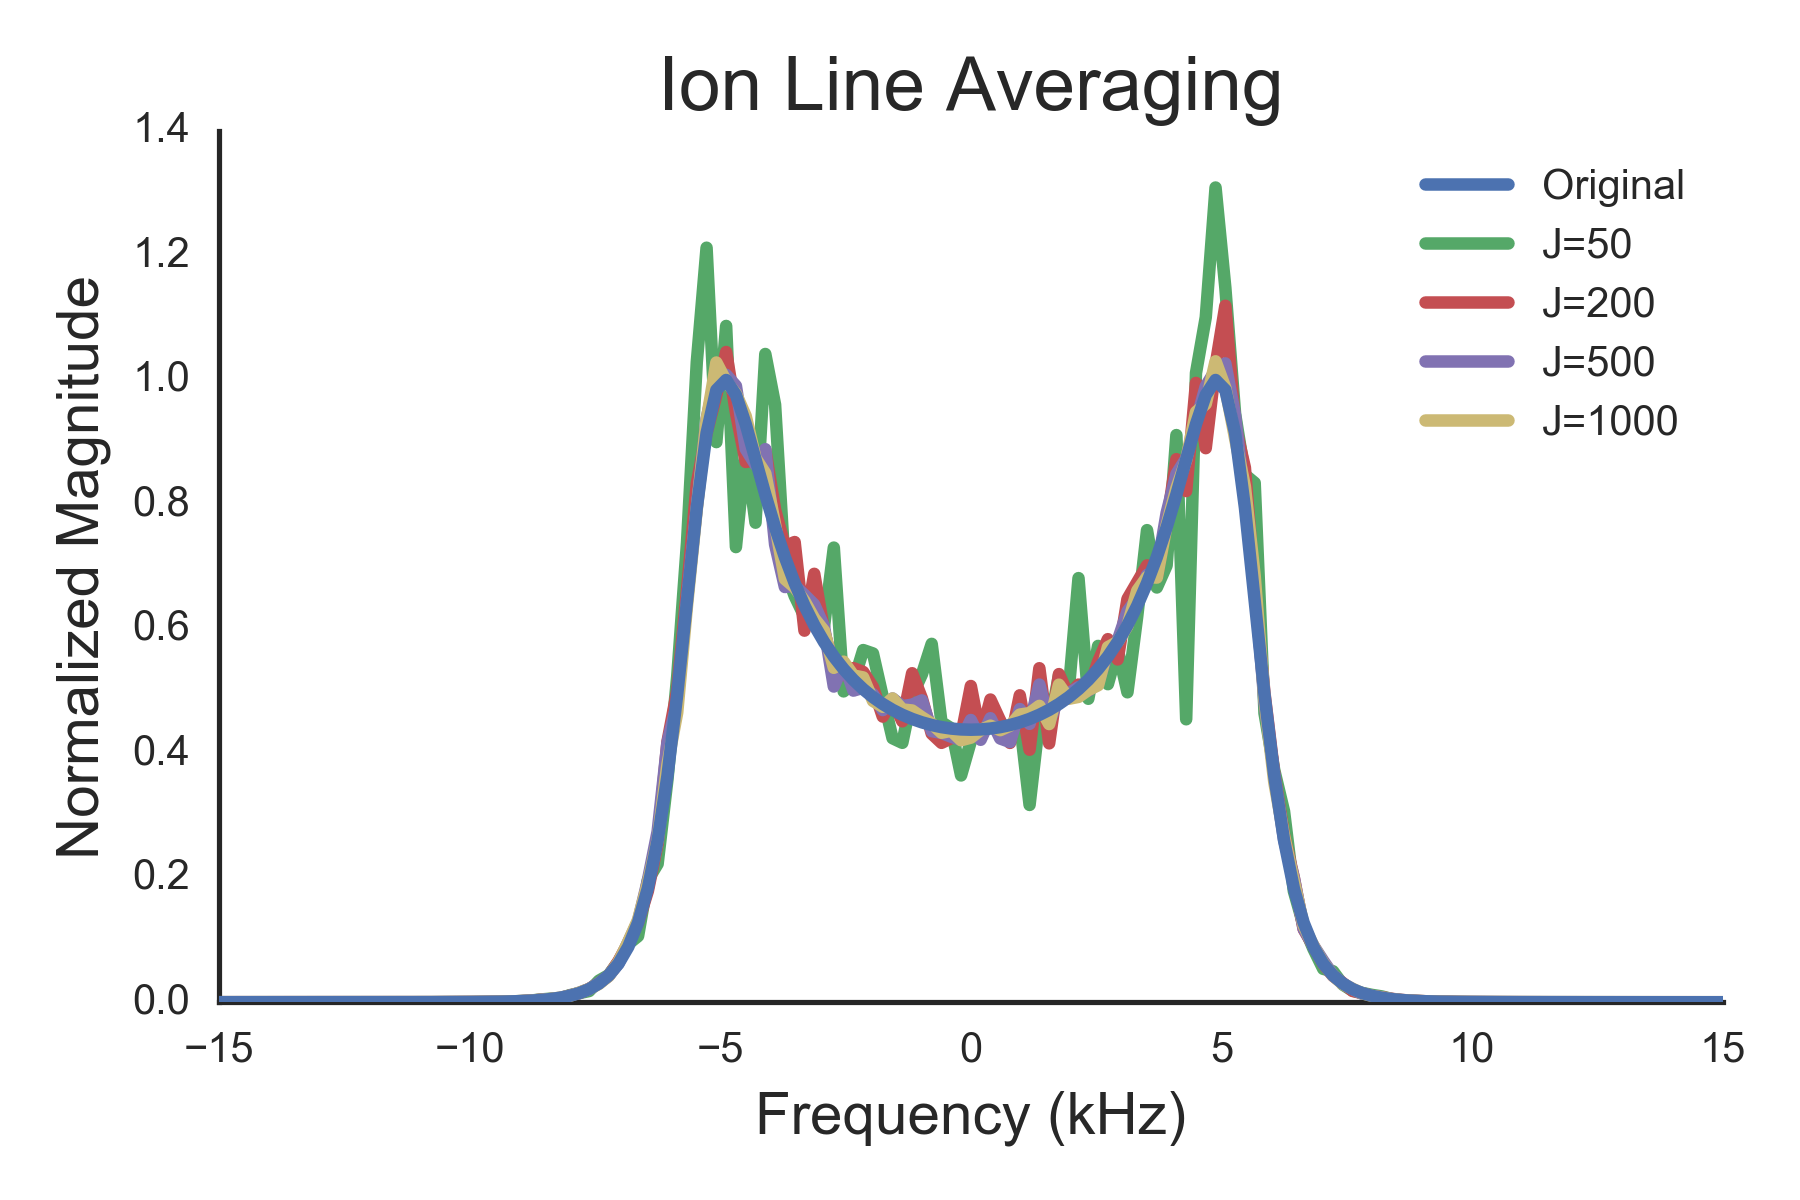
\includegraphics[width=4in]{Specionave}
\caption{IS spectrum ion line with all parameters from Figure \ref{fig:ispecch2} with $J =$ 50, 100, 500 and 1000 averaged realizations. }
\label{fig:ispecch2ave}
\end{figure}

\section{Radar Signal Processing}

ISR systems like other pulsed radar systems radiate a signal, $y(t)$, that can be represented as a finite length pulse, $s(t)$ modulated by a complex sinusoid
\begin{equation}
\label{eqn:sigone}
y(t)=s(t)e^{j2\pi f_0 t}
\end{equation}
where $f_0$ is the transmit frequency in Hz. Equivalently, $ f_0=c/\lambda_0$, where $\lambda_0$ is the wavelength of the transmitted wave and $c$ is the speed of light. The return signal reflected off of a target, which assuming for now has no motion may be modeled as
\begin{equation}
\label{eqn:sigone}
y_r(t)=A_0s(t-\Delta t)e^{j2\pi f_0 (t-\Delta t)}
\end{equation}
where $\Delta T$ round trip time and $A_0$ is an amplitude factor including propagation losses and target reflectivity \cite{richards2014fundamentals}. The radar system estimates the range $r$, or the distance between the target and sensor, by convention
\begin{equation}
\label{eqn:range_intro}
r=\frac{c\Delta T}{2}.
\end{equation}
Lastly, the signal is demodulated down to baseband, becoming
\begin{equation}
\label{eqn:baseband}
x(t)=A_0s(t-\Delta t)e^{-j2\pi\Delta t}
\end{equation}
Another key quantity estimated by ISR is the line of sight or Doppler velocity. The Doppler for this specific case acts as multiplication of the radar signal $s(t)$ with a simple single complex exponential
\begin{equation}
\label{simpledop}
x_d(t) = x(t)e^{j2\pi f_d t},
\end{equation}
 where $\omega_d$ is the Doppler frequency of the target. Assuming there are no relativistic effects this frequency can be represented as the following $f_d = 2v/\lambda_0 $, where $v$ is the velocity of the target. 

With ISR a distribution of electrons are probed, so we have an extremely large number of small cross-section targets within the beam. A better model would be a set of scatterers each with their weighted return and Doppler frequency, represented as
\begin{equation}
\label{multiDop}
\displaystyle x_d(t) = \sum_{n}^{N} x(t)V_ne^{j2\pi f_{n} t}.
\end{equation}
This model can be extended to a continuum of signals each with unique Doppler frequency, becoming
\begin{equation}
\label{conDop}
x_d(t) = \int x(t) V(f)e^{j2\pi ft} df.
\end{equation}
Pulling the $x(t)$ term out of the integral it is apparent that this is the Fourier transform of this relative weighting between each of the scatterers multiplied with the signal.  This is equivalent to a convolution in frequency space of the spectrum of the original radar signal and the Doppler spectrum with the collection of targets.  
The final form of the signal spectrum with Doppler added can be shown as the following
\begin{equation}
\label{finalDop}
x_d(t) = \int \left[\int X(\lambda)V(\lambda-f)d\lambda\right] e^{j\omega t}df.
\end{equation}
This shows that the measured Doppler on the radar signal can be formulated as the convolution of the Fourier transform of the radar signal along with the Doppler spectrum of the target.

This model can be extended from a single point to a much more general form spread across range
\begin{equation}
\label{eqn:scateqn}
x(t)= \int \int V(\mu,f)s(t-\mu)e^{j2\pi f t} d \mu df,
\end{equation}
where $V(\mu,\nu)$ is the scatter function and $\mu=2r/c$. One of the earlier uses of this form comes from the study of time varying communication channels \cite{Kailath:1962jx,Kailath:1963gh}. This scattering function drives the methodology on how the target can be properly measured. 
This model creates two classes of targets, distinguished by range bandwidth product. For the case of an an \textit{underspread} target
\begin{equation}
\label{eqn:trp}
B\frac{2r}{c}<1,
\end{equation}
where $B$ is the Doppler bandwidth \cite{Pfander:2015ea}. 
The case of the \textit{overspread} target occurs when this inequality does not hold.

\subsection{Doppler Measurement}

In this section, two methods of ISR pulse-Doppler measurement are examined. The pulse-Doppler method consists of the following steps:
\begin{enumerate}
\item radar sends a set of pulses that scatter off the targets 
\item target returns are binned into a two-dimensional array representing range and interpulse period (IPP)
\item a discrete Fourier transform (DFT) across pulses is taken to determine the Doppler spectrum \cite{richards2014fundamentals}. 
\item A power spectrum is formed by taking squared magnitude of the full range-Doppler map.  
\end{enumerate}
This pulse-Doppler processing method is commonly denoted \textit{coherent processing} \cite{richards2014fundamentals,richards2010principles,richards2014principles,skolnik2008radar}.
To avoid aliasing or Doppler folding, the pulse repetition frequency must be at least twice as large as largest Doppler frequency in the signal \cite{dtsp:openhiem}. 

An alternative Doppler processing method replaces steps \#2 and \#3 with a measurement of the autocorrelation function (ACF) within the IPP and a DFT across the lags is taken to get the Doppler spectrum.
The formation of this spectrum is the same as forming Wigner-Ville distribution along range \cite{TFAcohen}.
Because phase coherency is not needed across pulses this is considered an \text{incoherent processing} technique \cite{richards2014fundamentals,richards2010principles,richards2014principles,skolnik2008radar}. 
Note that ISR received its name due to the physical definition of incoherent scatter as explained in Section \ref{sec:incohscat} \cite{gordon58,dougherty:farley1960}.

Both of these measurement methods have trade offs. Using the pulse-Doppler method, a phase-coherent signal that is relatively narrow in frequency can obtain a large amount of gain compared to the background noise. The Doppler bandwidth that can be view unambiguously will be tied to the PRF. The issue of range ambiguity can arise if the support of the target is further in range than a single pulse can travel in an IPP. The maximum unambiguous range, $r_a$, can be represented as 
\begin{equation}
\label{eqn:maxuar}
r_a =  \frac{cT}{2}
\end{equation}
where $T$ is the IPP time. 
The method using the Wigner-Ville distribution for the spectrum formation will not give nearly as much gain but it can form a much more broadband spectrum without having to decrease the unambiguous range~\cite{richards2014fundamentals}.

When designing a moving target indicator (MTI) radar system the target scattering function can be approximated as a Dirac delta or a compactly supported function in range and Doppler \cite{richards2014fundamentals}. 
These types are generally underspread as their range extent and Doppler bandwidth follows the inequality in~\eqref{eqn:trp}. 
The ionosphere is not compactly supported in range if one wants to do F-region studies, which can stretch from 150-700 km in altitude. 
Using the spectrum in Figure~\ref{fig:ispecch2}, it can be seen that the signal is at least 20kHz in bandwidth.
This broad bandwidth requires the same PRF for unambitious sampling. 
This would yield only 7.5~km of unambiguous range so it is necessary to use the Wigner-Ville distribution method on this overspread target. 


 %There are still cases of ISR systems that use a pulses Doppler technique, but these are generally relegated to D-region studies where the necessary unambiguous range is lower and the spectrums are narrower.


%%%%%%%%%%%%%% Processing %%%%%%%%%%%%%%%%%%%%%%%%%%%%%%%
\section{ISR Processing}\label{section:isrproc}
After complex receiver voltage data have been received, the data are processed to create estimates of the ACF at desired points of space \cite{farley1969,nygren1996}. This processing follows the flow chart presented in Figure \ref{fig:chain}.  Note that we assume here a signal pipeline which creates a single altitude measurement for analysis.  More sophisticated approaches for ISR analysis exist that use information from multiple altitudes, including full profile analysis \cite{RDS:RDS3308}, lag profile inversion \cite{Virtanen:20082vx}, and others, but treatment of these approaches is beyond the scope of this chapter.

\begin{figure}[!t]
\centering
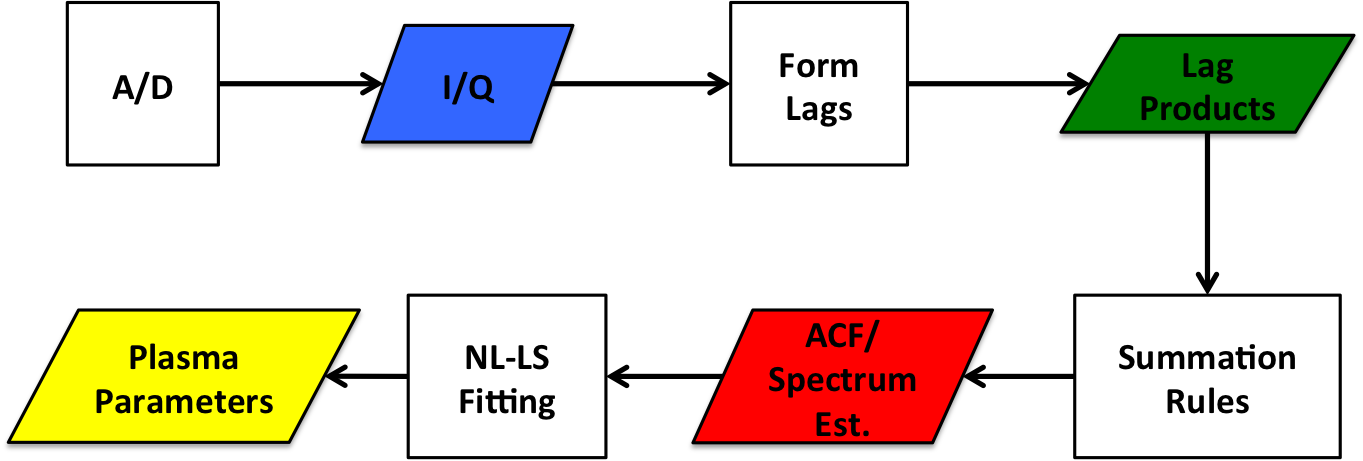
\includegraphics[width=5.5in]{datastackchain}
\caption{ISR signal processing chain, with signal processing operations as squares and data products as diamonds.}
\label{fig:chain}
\end{figure}


The lag product formation is an initial estimate of the autocorrelation function. The sampled complex receiver voltage can be represented as $x(n) \in\mathbb{C}^N$ where $N$ is the number of samples in an inter-pulse period. For each range gate $m\in 0,1,...M-1$ a complex autocorrelation is estimated for each lag of $l \in 0,1...,L-1$.  To get better statistics this operation is performed for each pulse $j\in 0,1,...J-1$ and then summed over $J$ independent pulses. The entire operation to form the initial estimate of $\widehat{R}(m,l)$ may be expressed as

\begin{equation}
\label{eq:lagpro}
\widehat{R}(m,l) = \displaystyle\sum\limits_{j=0}^{J-1} x(m-\lfloor l/2\rfloor,j)x^*(m+\lceil l/2 \rceil,j).
\end{equation}

The case shown in Equation \ref{eq:lagpro} is a centered lag product.  Other types of lag product calculations are available but a centered product is most common. For this case, the range gate index $m$ and sample index $n$ can be related by $m=n-\lfloor L/2\rfloor$ and the maximum lag and sample relation is $M=N-\lceil L/2 \rceil$.  This lag product formation is the first step in computing a discrete Wigner Distribution \cite{TFAcohen}. This  step adds a bias to the ACF estimate which acts as a weighting on larger lags, represented as $\mathcal{W}(l)$ where weighting can be calculated from details of the range-lag ambiguity function. The expected value for the estimator, assuming the use of a simple uncoded pulse waveform, becomes

\begin{equation}
\label{eq:lagprobias}
\left\langle\widehat{R}(m,l) \right\rangle = \mathcal{W}(l)R(m,l) =\frac{L-l}{L}R(m,l).
\end{equation}

%This specific type of lag product formation is detailed in \cite{farley1969} and had been referred to as unbiased. This terminology does differ from what is used in statistic signal processing literature such as \cite{randomsigshanmugan} where the unbiased autocorrelation function estimate is carried out as so,
%
%\begin{equation}
%\label{eq:lagproub}
%\hat{R}(m,l) = \frac{1}{L-l}\displaystyle\sum\limits_{j=0}^{J-1} x(m-\lfloor l/2\rfloor,j)x^*(m+\lceil l/2 \rceil,j).
%\end{equation}
%
%\noindent With out the $\frac{1}{L-l}$ term the estimator will be windowed with a triangular function thus impacting the estimate of the ISR spectrum as this will act as a convolution in the frequency domain. This bias is taken into account in \cite{farley1969} but it is simply wrapped up into the ambiguity function. 

Applying a summation rule is generally the next step in creating an estimate of the autocorrelation function for single altitude analysis. This is done for a number of reasons, but primarily to improve estimate statistics.  Furthermore, if the right rule is chosen, then the range ambiguity can be made approximately constant across the lags, which can make inversions easier \cite{nygren1996}. Summation rules based on other criteria can be used but our simulations use the trapezoidal summation, which is a common choice and leads to uniform range resolution across all lags. It can be represented as follows:

\begin{equation}
\label{eq:sumrule}
\widehat{R}_s(m,l) = \displaystyle\sum\limits_{i=-((v-1)/2+\lceil l/2 \rceil)}^{((v-1)/2+\lfloor l/2\rfloor)} \widehat{R}(m+i,l),
\end{equation}

\noindent where $v$ is the 'volume' index or the number of gates integrated at zero lag (restricted to positive odd integers here) and $\widehat{R}_s(m,l)$ is the final ACF estimate after the summation rule \cite{nygren1996}. 
% pcom checked for variables, already defined
However, the final result of this summation rule will still lead to a statistically biased ACF. For the uncoded waveform case, this summation rule leads to the following expected value for the estimator \cite{nygren1996},

\begin{equation}
\label{eq:sumruleest}
\left\langle\widehat{R}_s(m,l) \right\rangle  =\frac{v+l}{v\mathcal{W}(0)}\mathcal{W}(l)R(m,l) =\left(-\frac{1}{vL}l^2+\frac{L-v}{Lv}l+1\right)   R(m,l).
\end{equation}

An example summation rule for a central product is shown in Figure \ref{fig:sumrule}.The image on the left is a basic representation of an ambiguity function of a long pulse and is mirrored on the right with red bars which would show the integration area under it so the ambiguity function for each lag will be of equal size in range. There are a number of different summing rule each with their own trade offs \cite{nygren1996}.

\begin{figure}[!t]
\centering
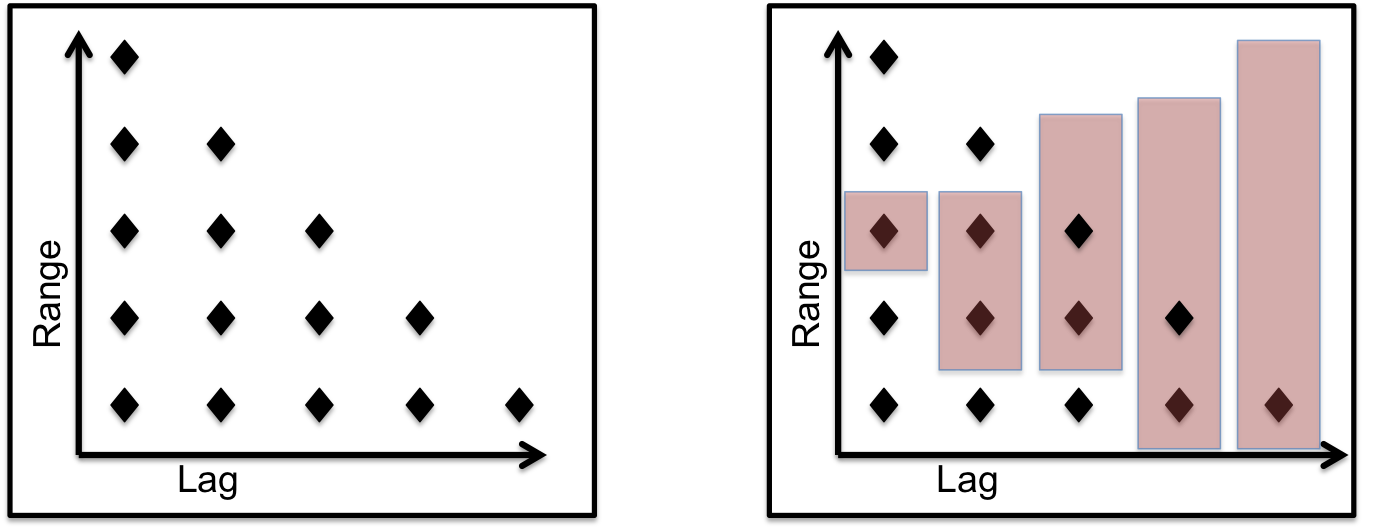
\includegraphics[width=3in]{sumrule}
\caption{Summation Rule Diagram}
\label{fig:sumrule}
\end{figure}

%In the processing this is basically a summing of lags from different ranges. The amount of summing is similar to what is shown in Figure \ref{fig:sumrule}.   



%\begin{equation}
%\label{eq:lagpronoise}
%\hat{R}_w(m,l) = \displaystyle\sum\limits_{j=0}^{J-1} w(m_w-\lfloor l/2\rfloor,j)w^*(m_w+\lceil l/2 \rceil,j),
%\end{equation}

Finally, noise effects are included by subtracting an estimate of the noise correlation from $\widehat{R}_s(m,l)$.  We represent the noise correlation function as $\widehat{R}_w(m,l)$, the ACF estimate of the background noise process of the radar $w(n_w)$ using the steps in Equations \ref{eq:lagpro} and \ref{eq:sumrule}. In a real radar system the noise process is typically sampled either during a calibration period for the radar when nothing is being emitted, or at ranges sufficiently distant that scattered ionospheric signal is assumed to be negligible. The final estimate of the autocorrelation function after the noise subtraction and summation rule is represented by $\widehat{R}_f(m,l)$.

Along with the first order moment of the ACF seen in \ref{eq:sumruleest}, in order to do error analysis a second order moment is needed. The covariance matrix between each lag estimate can be formed using the formulation in Equation 2 of \cite{hysell2008}, rewritten here as

\begin{equation}
\label{eqn:covcalc}
C_{\tau_1,\tau_2} = \frac{1}{2J} \left( \ R(0)  R^*(\tau_1-\tau_2) +  R(\tau_1) R^*(\tau_2) \right),
\end{equation}

\noindent where, $R(\tau)$ is the estimated ACF as a function of lag $\tau$, $C_{\tau_1,\tau_2}$ is the entry in the covariance matrix of the estimated ACF at lags $\tau_1$ and $\tau_2$,  and $J$ is the number of samples or pulses averaged together to create the estimate. The diagonals of this matrix can be thought of as the autocovariances of each of the lags.  Along these diagonals, by setting $\tau_2 = \tau_1 \equiv \tau$, Equation \ref{eqn:covcalc} simplifies to

\begin{equation}
\label{eqn:covdiag}
C_{\tau,\tau} = \frac{1}{2J} \left(  |R(0)|^2 +|R(\tau)|^2\right).
\end{equation}

The variance of the signal ACF estimate is further increased once sensor and sky noise is added.  If the noise is assumed to be uncorrelated with the signal, the error from the noise, $\left|R_w (\tau)\right|^2$ (e.g. the square of the noise ACF) can be added to the error from the inherent fluctuations in the signal, and the autocovariance expression becomes

\begin{equation}
\label{eqn:covdiagwn}
C_{\tau,\tau} = \frac{1}{2J} \left(  |R(0)|^2 +|R(\tau)|^2 + \left|R_w (0)\right|^2+\left|R_w (\tau)\right|^2\right).
\end{equation}


After the final estimation of the spectrum is complete, nonlinear least squares fitting takes place to determine plasma parameters.  
%\pcom{This entire section can be collapsed to one reference and saved for the thesis chapter.}%
%{
The class of nonlinear least squares problems relevant to ISR parameter estimation can be represented as the minimization of a cost function of the form \cite{kayvol1},

\begin{equation}
	\mathbf{\hat{p}}= \underset{\mathbf{p}}{\text{argmin}} (\mathbf{y}-\bm{\theta}(\mathbf{p}))^*\mathbf{C}_{\mathbf{y}}^{-1}(\mathbf{y}-\bm{\theta}(\mathbf{p})).
\label{nlls}
\end{equation}

In Equation \ref{nlls}, the data represented as $\mathbf{y}$ would be the final estimate of the ACF $\widehat{R}_f(m,l)$ at a specific range, or its spectrum $\widehat{S}_f(m,\omega)$. The matrix $\mathbf{C}_{\mathbf{y}}$  is the covariance matrix from the ACFs or spectra depending on what is being fit. The covariance matrix for the ACF is detailed in Equation \ref{eqn:covcalc}, while the covariance matrix of the spectra is simply the ACF matrix but with discrete Fourier Transforms applied to the rows and columns. The parameter vector $\mathbf{P}$ would be the plasma parameters $N_e$, $T_e$, $T_i$ and $V_i$. The fit function, $\bm{\theta}$, is the IS spectrum calculated from a models \cite{kudeki:milla:1} and smeared by the ambiguity function. In the case of the long pulse the ambiguity can be simply applied by multiplying it with the autocorrelation function $R(l)$ if the summation rule is properly applied. As in previous publications, \cite{nikoukar2008}, the Levenberg-Marquardt algorithm is used to fit the plasma parameters to the ACFs or spectra \cite{levenberg1944,marquardt:1963}.

The last step is to calculate the errors in the parameter estimates. In order to do this a numerical approximation is computed of the Jacobian matrix between the data and the ACF, $\mathbf{J}$, at $\mathbf{p}=\mathbf{\hat{p}}$. Given this Jacobian, the formula to estimate the parameter error matrix, $\mathbf{C}_{\mathbf{\hat{p}}}$ according to \cite{Hysell:2000cq}, is

\begin{equation}
\label{eqn:jacinv}
\mathbf{C}_{\mathbf{\hat{p}}}=(\mathbf{J}^T \mathbf{C}^{-1}\mathbf{J})^{-1},
\end{equation}
%\begin{equation}
%\label{eqn:jacinv}
%\bm{\Sigma}_{\mathbf{\hat{p}}}=\frac{(\mathbf{J}^T\mathbf{J})^{-1} (\mathbf{y}-\bm{\theta}(\mathbf{\hat{p}}))^*\bm{\Sigma}^{-1}(\mathbf{y}-\bm{\theta}(\mathbf{\hat{p}}))}{L-N_{\mathbf{p}}},
%\end{equation}

\noindent  The variances of the parameters are then taken as the diagonals of the matrix. 

%The correlation matrix $\bm{\Sigma}$ is often realized as a diagonal matrix for many ISR systems the variance of the lags or each point of the spectrum being the values. The variance of the ACF estimator can be estimated using the following,
%
%\begin{equation}
%\label{eqn:acfvar}
%\sigma_{\hat{R}(l)}^2=\frac{1}{JL}\displaystyle \sum_{m=-(L-l-1)}^{L-l-1}\left(\frac{L-|m|+1}{L}\right)\left(|\hat{R}(m)|^2 +|\hat{R}(m+l)\hat{R}(m-l)|\right) + \hat{N}^2
%\end{equation}
%
%\noindent where $N$ is the estimated noise power. To estimate the spectrum variance the matrix $\bm{\Sigma}$ is transformed in to the Fourier domain using FFTs (FFT on the columns and IFFT on the rows) so as to model the $\mathbf{F}\bm{\Sigma} \mathbf{F}^*$ matrix operation. 



%%
The diagonal values usually used, noted as $\mathbf{c}_i^2$, usually the same unless there is a larger measurement error for one of the lags or spectrums. The following formula from  \cite{nicollsisrschool2013} can be used:

\begin{equation}
\label{sigpow}
\sigma_i = \frac{S}{\sqrt{J}}\left(1+\frac{1}{SNR}\right).
\end{equation}

\noindent where $S$ is the signal power and $SNR$ is the signal to noise ratio. The noise level can be estimated from the calibration period. 

In the past, ISR researchers have used the Levenberg-Marquart algorithm to fit data \cite{nikoukar2008}. This specific iterative algorithm moves the parameter vector $\mathbf{p}$ by a perturbation $\mathbf{h}$ at each iteration\cite{gavin:2013}. Specifically Levenberg-Marquart was designed to be a sort of meld between two different methods Gradient Decent, and Gauss-Newton. The perturbation vector $\mathbf{h}_{lm}$ can be calculated using the following:

\begin{equation}
\left[ \mathbf{J}^T\bm{\Sigma}^{-1}\mathbf{J}\right]\mathbf{h}_{lm} =\mathbf{J}^T\bm{\Sigma}^{-1}(\mathbf{y}-\bm{\theta}(\mathbf{p}))
\label{hlm}
\end{equation}

\noindent where $\mathbf{J}$ is the Jacobian matrix $\partial \bm{\theta}/\partial \mathbf{p}$ \cite{levenberg1944,marquardt:1963}. 

%Using the covariance matrix from the fitted parameters, an overall error estimate can be achieved. This matrix is calculated using a numerical approximation to the Jacobian matrix that the function uses to determine the solution. The Hessian, $\mathbf{H}$ is then calculated by using the Jacobian and then inverted to get the covariance matrix. Due to the way the numerical routines solve the problem, this matrix must be multiplied by the error between the estimated parameters and the data,
%
%\begin{equation}
%\label{eqn:jacinv}
%\bm{\Sigma}_{\mathbf{\hat{p}}}=\frac{(\mathbf{J}^T\mathbf{J})^{-1} (\mathbf{y}-\bm{\theta}(\mathbf{\hat{p}}))^*\bm{\Sigma}^{-1}(\mathbf{y}-\bm{\theta}(\mathbf{\hat{p}}))}{L-N_{\mathbf{p}}},
%\end{equation}

%\noindent where $N_{\mathbf{p}}$ is the number of parameters being fit. The variances of the parameters are then taken as the diagonals of the matrix.}

 %If the Hessian matrix is undefined so it can not be inverted and a proper estimate of the errors is not possible.

